% !TEX root = ./main.tex
%%%%%%%%%%%%%%%%%%%%%%%%%%%%%%%%%%%%%%%%%%%%%%%%%%%%%%%%%%%%%%%%%%%%%%%%%%%%%%%%%%%%%%%%%%
% Dans cette section, indiquez et décrivez tous les Invariants nécessaires.              %
%                                                                                        %
% Pour chaque SP nécessitant un Invariant (une sous-section/SP):                         %
% - Donnez l'Invariant Graphique                                                         %
% - Donnez l'Invariant Formel correspondant à l'Invariant Graphique                      %
% Pensez à utiliser les notations définies précédemment.                                 %
%%%%%%%%%%%%%%%%%%%%%%%%%%%%%%%%%%%%%%%%%%%%%%%%%%%%%%%%%%%%%%%%%%%%%%%%%%%%%%%%%%%%%%%%%%
\section{Invariants}\label{invariants}
%%%%%%%%%%%%%%%%%%%%

\subsection{SP1:}
\textbf{Invariant formel:} \\
    $0 < k < N$ \\
    $\land$ \\
    $T[0..k-1] \neq T[N-k..N-1]$ \\

\begin{figure}[h]
    \centering
    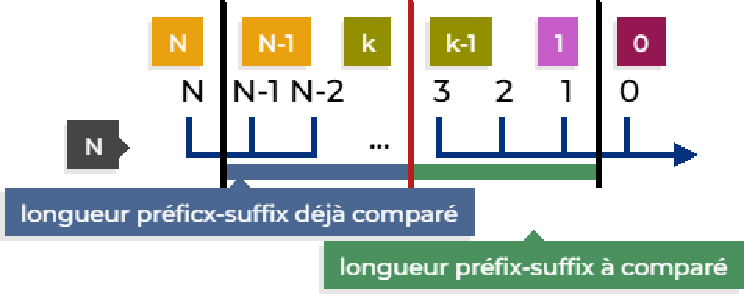
\includegraphics[width=0.7\textwidth]{invariant_1.pdf}
    \caption{Invariant graphique SP1}
\end{figure}

\subsection{SP2:}
\textbf{Invariant formel:} \\
    $T = T_0 \land k = k_0$ \\
    $\land$ \\
    $0 \leq i < k$ \\
    $\land$ \\
    $T[i] = T[N - k + i]$ \\

\begin{figure}[h]
    \centering
    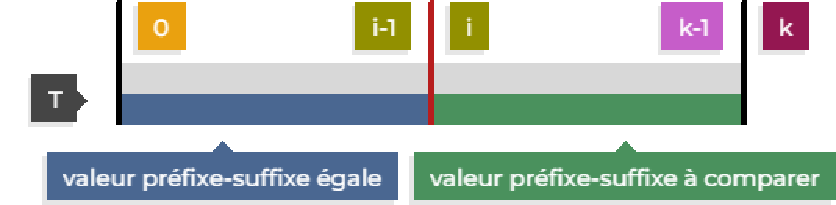
\includegraphics[width=0.7\textwidth]{invariant_2.pdf}
    \caption{Invariant graphique SP2}
\end{figure}

